\documentclass[a4paper]{tufte-handout}
% Shared preamble for all lab reports (Tufte handout layout).
%
% Usage, from labN/report/labN_report.tex:
%   \documentclass[a4paper,justified]{tufte-handout}
%   % Shared preamble for all lab reports (Tufte handout layout).
%
% Usage, from labN/report/labN_report.tex:
%   \documentclass[a4paper,justified]{tufte-handout}
%   % Shared preamble for all lab reports (Tufte handout layout).
%
% Usage, from labN/report/labN_report.tex:
%   \documentclass[a4paper,justified]{tufte-handout}
%   \input{../../report-style/preamble}
%   \labtitle{2}{ROS, TF and Quaternions}
%
% Build: latexmk -pdf labN_report.tex

\usepackage{amsmath,amssymb,bm}
\usepackage{booktabs,tabularx,array}
\usepackage{graphicx}
\usepackage{xcolor}
\usepackage{textcomp}
\usepackage{listings}
\usepackage[most]{tcolorbox}
\usepackage{siunitx}
\usepackage{cleveref}

\setcounter{secnumdepth}{2}
\crefname{section}{Section}{Sections}
\crefname{figure}{Figure}{Figures}
\crefname{table}{Table}{Tables}
\crefname{listing}{Listing}{Listings}
% In main-column table/figure floats a \label after \caption refers to the
% section (tufte-latex with the current kernel); write
% \caption{Text.\protect\label{key}} instead. Margin floats are unaffected.
\hypersetup{colorlinks=true, allcolors=[rgb]{0.12,0.25,0.55}}

% --- Author and course -------------------------------------------------------
\newcommand{\studentname}{Xuanye Xu}
\newcommand{\studentids}{24020036071 / H00490299}
\newcommand{\coursename}{Robotics Integration I --- VNAV Labs}

% \labtitle{<lab number>}{<topic>}
\newcommand{\labtitle}[2]{%
  \title[Lab #1: #2]{Lab #1 Report: #2}%
  \author[\studentname]{\studentname\\[2pt]
    {\normalsize\normalfont Student ID \studentids\\ \coursename}}%
  \date{\today}}

% --- Grading items -----------------------------------------------------------
% \gradeditem{<label>}{<title>}{<points>} starts a section for one grading item.
\newcommand{\gradeditem}[3]{%
  \section{#2\texorpdfstring{\enspace{\normalfont\small[#3~pts]}}{ [#3 pts]}}\label{#1}}

% Evidence summary shown at the end of each graded section.
\newtcolorbox{evidence}{enhanced, breakable, frame hidden, arc=0pt,
  colback=black!4, borderline west={1.2pt}{0pt}{black!55},
  left=6pt, right=4pt, top=3pt, bottom=3pt,
  before upper={\textsc{Evidence}\quad}}

% Marks unfinished content in red; a final report must contain none.
\newcommand{\pending}[1]{\textcolor{red}{[PENDING: #1]}}

% --- Code and terminal output ------------------------------------------------
\lstdefinestyle{code}{language=C++, basicstyle=\ttfamily\footnotesize,
  keywordstyle=\bfseries, commentstyle=\itshape\color{black!60},
  numbers=left, numberstyle=\tiny\color{black!50}, xleftmargin=1.5em,
  columns=fullflexible, keepspaces, breaklines, showstringspaces=false,
  upquote=true}
\lstdefinestyle{log}{basicstyle=\ttfamily\scriptsize, frame=leftline,
  framerule=0.6pt, rulecolor=\color{black!40}, xleftmargin=0.8em,
  columns=fullflexible, keepspaces, breaklines, upquote=true}
\lstset{style=log}

%   \labtitle{2}{ROS, TF and Quaternions}
%
% Build: latexmk -pdf labN_report.tex

\usepackage{amsmath,amssymb,bm}
\usepackage{booktabs,tabularx,array}
\usepackage{graphicx}
\usepackage{xcolor}
\usepackage{textcomp}
\usepackage{listings}
\usepackage[most]{tcolorbox}
\usepackage{siunitx}
\usepackage{cleveref}

\setcounter{secnumdepth}{2}
\crefname{section}{Section}{Sections}
\crefname{figure}{Figure}{Figures}
\crefname{table}{Table}{Tables}
\crefname{listing}{Listing}{Listings}
% In main-column table/figure floats a \label after \caption refers to the
% section (tufte-latex with the current kernel); write
% \caption{Text.\protect\label{key}} instead. Margin floats are unaffected.
\hypersetup{colorlinks=true, allcolors=[rgb]{0.12,0.25,0.55}}

% --- Author and course -------------------------------------------------------
\newcommand{\studentname}{Xuanye Xu}
\newcommand{\studentids}{24020036071 / H00490299}
\newcommand{\coursename}{Robotics Integration I --- VNAV Labs}

% \labtitle{<lab number>}{<topic>}
\newcommand{\labtitle}[2]{%
  \title[Lab #1: #2]{Lab #1 Report: #2}%
  \author[\studentname]{\studentname\\[2pt]
    {\normalsize\normalfont Student ID \studentids\\ \coursename}}%
  \date{\today}}

% --- Grading items -----------------------------------------------------------
% \gradeditem{<label>}{<title>}{<points>} starts a section for one grading item.
\newcommand{\gradeditem}[3]{%
  \section{#2\texorpdfstring{\enspace{\normalfont\small[#3~pts]}}{ [#3 pts]}}\label{#1}}

% Evidence summary shown at the end of each graded section.
\newtcolorbox{evidence}{enhanced, breakable, frame hidden, arc=0pt,
  colback=black!4, borderline west={1.2pt}{0pt}{black!55},
  left=6pt, right=4pt, top=3pt, bottom=3pt,
  before upper={\textsc{Evidence}\quad}}

% Marks unfinished content in red; a final report must contain none.
\newcommand{\pending}[1]{\textcolor{red}{[PENDING: #1]}}

% --- Code and terminal output ------------------------------------------------
\lstdefinestyle{code}{language=C++, basicstyle=\ttfamily\footnotesize,
  keywordstyle=\bfseries, commentstyle=\itshape\color{black!60},
  numbers=left, numberstyle=\tiny\color{black!50}, xleftmargin=1.5em,
  columns=fullflexible, keepspaces, breaklines, showstringspaces=false,
  upquote=true}
\lstdefinestyle{log}{basicstyle=\ttfamily\scriptsize, frame=leftline,
  framerule=0.6pt, rulecolor=\color{black!40}, xleftmargin=0.8em,
  columns=fullflexible, keepspaces, breaklines, upquote=true}
\lstset{style=log}

%   \labtitle{2}{ROS, TF and Quaternions}
%
% Build: latexmk -pdf labN_report.tex

\usepackage{amsmath,amssymb,bm}
\usepackage{booktabs,tabularx,array}
\usepackage{graphicx}
\usepackage{xcolor}
\usepackage{textcomp}
\usepackage{listings}
\usepackage[most]{tcolorbox}
\usepackage{siunitx}
\usepackage{cleveref}

\setcounter{secnumdepth}{2}
\crefname{section}{Section}{Sections}
\crefname{figure}{Figure}{Figures}
\crefname{table}{Table}{Tables}
\crefname{listing}{Listing}{Listings}
% In main-column table/figure floats a \label after \caption refers to the
% section (tufte-latex with the current kernel); write
% \caption{Text.\protect\label{key}} instead. Margin floats are unaffected.
\hypersetup{colorlinks=true, allcolors=[rgb]{0.12,0.25,0.55}}

% --- Author and course -------------------------------------------------------
\newcommand{\studentname}{Xuanye Xu}
\newcommand{\studentids}{24020036071 / H00490299}
\newcommand{\coursename}{Robotics Integration I --- VNAV Labs}

% \labtitle{<lab number>}{<topic>}
\newcommand{\labtitle}[2]{%
  \title[Lab #1: #2]{Lab #1 Report: #2}%
  \author[\studentname]{\studentname\\[2pt]
    {\normalsize\normalfont Student ID \studentids\\ \coursename}}%
  \date{\today}}

% --- Grading items -----------------------------------------------------------
% \gradeditem{<label>}{<title>}{<points>} starts a section for one grading item.
\newcommand{\gradeditem}[3]{%
  \section{#2\texorpdfstring{\enspace{\normalfont\small[#3~pts]}}{ [#3 pts]}}\label{#1}}

% Evidence summary shown at the end of each graded section.
\newtcolorbox{evidence}{enhanced, breakable, frame hidden, arc=0pt,
  colback=black!4, borderline west={1.2pt}{0pt}{black!55},
  left=6pt, right=4pt, top=3pt, bottom=3pt,
  before upper={\textsc{Evidence}\quad}}

% Marks unfinished content in red; a final report must contain none.
\newcommand{\pending}[1]{\textcolor{red}{[PENDING: #1]}}

% --- Code and terminal output ------------------------------------------------
\lstdefinestyle{code}{language=C++, basicstyle=\ttfamily\footnotesize,
  keywordstyle=\bfseries, commentstyle=\itshape\color{black!60},
  numbers=left, numberstyle=\tiny\color{black!50}, xleftmargin=1.5em,
  columns=fullflexible, keepspaces, breaklines, showstringspaces=false,
  upquote=true}
\lstdefinestyle{log}{basicstyle=\ttfamily\scriptsize, frame=leftline,
  framerule=0.6pt, rulecolor=\color{black!40}, xleftmargin=0.8em,
  columns=fullflexible, keepspaces, breaklines, upquote=true}
\lstset{style=log}

\labtitle{3}{Trajectory Tracking with a Geometric Controller}
\author[\studentname]{\studentname\\[2pt]
  {\normalsize\normalfont Student ID \studentids\quad Group~7\\ \coursename}}

% clickable path of a file in the public repository
\newcommand{\repo}[1]{\href{https://github.com/Qzz139/LEARN-MIT16.485/blob/main/#1}{\nolinkurl{#1}}}

\begin{document}
\maketitle

\begin{abstract}
A geometric tracking controller on $\mathrm{SE}(3)$ was implemented
for the simulated quadrotor of the MIT VNAV Lab~3 and tuned to follow a circle of
radius \SI{5}{m} at \SI{2}{m} altitude.
With the final gains $(k_x,k_v,k_R,k_\Omega)=(8,5,10,2)$ the position error is
\SI{4.3}{cm} RMS and the pitch jitter \SI{0.26}{\degree}, and the drone's yaw
trails the rotating \texttt{av-desired} frame by \SI{5.86}{\degree}, close to the
\SI{5.74}{\degree} predicted from the control law.
Gains chosen on tracking error alone reached \SI{1.8}{cm} but made the rotors
chatter and reverse, and were rejected.
\end{abstract}

\section*{Grading Map}

\begin{table*}[h]
\small
\begin{tabularx}{\linewidth}{@{}l l r l X@{}}
\toprule
Part & Grading item & Points & Section & Evidence \\
\midrule
Individual & Deliverable 1: transformations & 25 & \cref{sec:d1} & One-line answers; output of a check program \\
Individual & Deliverable 2: modelling and control & 25 & \cref{sec:d2} & $F$ matrices and their ranks; drag compensation \\
Team & ROS communication & 10 & \cref{sec:ros} & Node graph; topic rates; frame of the odometry twist \\
Team & Controller (code body) & 20 & \cref{sec:ctrl} & Control law and code; circle tracking; RViz video \\
Team & \texttt{av-desired} rotation & 10 & \cref{sec:yaw} & RViz sequence; yaw tracking and a model of its lag \\
Team & Gain tuning & 10 & \cref{sec:tune} & 36 logged runs; error and smoothness table; video \\
\bottomrule
\end{tabularx}
\end{table*}

\section{Lab Introduction and Team Information}\label{sec:intro}
The lab implements the geometric controller of Lee et al.,\cite{lee2010} which
turns a desired trajectory (position, velocity, acceleration and yaw) into the
four rotor speeds of a quadrotor in the TESSE Unity simulator, tunes it on a
circular trajectory, and adds two individual exercises on rotation conventions
and quadrotor modelling.\cite{vnav2023lab3}
The code is the \texttt{VNAV2023} release of the lab template.\cite{vnavlabs}
\marginnote{The course page links the 2021 release, which for this lab differs only
in the move of the trajectory publisher to \texttt{tf2} and one Python requirement;
the downloadable simulator matches 2023. Environment: WSL~2 Ubuntu 20.04.6, ROS
Noetic, simulator rendering on an RTX~4070~SUPER through D3D12. Commands that
reproduce every item: \repo{lab3/HUMANS.md}.}
Group~7 has one member; the code, the experiments and the draft of this report
were done with the help of an AI assistant (Claude, by Anthropic),\cite{claude} and
the author reviewed all results reported here.
\Cref{sec:d1,sec:d2} are the individual deliverables and
\cref{sec:ros,sec:ctrl,sec:yaw,sec:tune} the team experiment.

\gradeditem{sec:d1}{Deliverable 1: Transformations in Practice}{25}
The deliverable asks for one-line conversions between a
\texttt{geometry\_msgs::Quaternion} and a \texttt{tf2::Quaternion}, the scalar part
of a quaternion, its yaw, and a $3\times3$ Eigen rotation matrix built from a
message. The answers (from the headers \texttt{tf2\_geometry\_msgs},
\texttt{tf2/utils.h} and \texttt{tf2\_eigen}):

\begin{lstlisting}[style=code]
tf2::fromMsg(quat_msg, quat_tf);                           // A.1
geometry_msgs::Quaternion quat_msg = tf2::toMsg(quat_tf);  // A.2
quat_tf.getW();                                            // A.3
tf2::getYaw(quat_t);                                       // B.1
Eigen::Quaterniond q;  tf2::fromMsg(quat_msg, q);          // B.2
Eigen::Matrix3d R = q.toRotationMatrix();
\end{lstlisting}

A check program runs every line on the rotation with roll, pitch and yaw
$(0.1,-0.2,0.7)$\,rad: the quaternion survives the round trip, \texttt{getYaw}
returns 0.700000, and the Eigen matrix matches \texttt{tf2::Matrix3x3} exactly.

\begin{evidence}
\repo{lab3/scripts/d1_tf2_check.cpp} and its output
\repo{lab3/results/logs/d1_tf2_check.txt}.
\end{evidence}

\gradeditem{sec:d2}{Deliverable 2: Modelling and Control of UAVs}{25}

\paragraph{(A) Structure of quadrotors.}
Rotor $i$ at $(x_i,y_i)$, spinning in direction $s_i=\pm1$ ($+1$ counter-clockwise
seen from above), adds $c_f u_i$ to the thrust, $c_f y_i u_i$ and $-c_f x_i u_i$ to
the roll and pitch torques and $-s_i c_d u_i$ to the yaw torque, with
$u_i=\omega_i|\omega_i|$; so $(f,\tau_x,\tau_y,\tau_z)^\top=F\,u$.
In the figure of the exercise the rotors sit at
$(x_i,y_i)=a\,(-1,1),\,a\,(-1,-1),\,a\,(1,-1),\,a\,(1,1)$ with $a=d/\sqrt2$, and
quadrotor (a) has $s=(1,-1,1,-1)$:
\begin{equation*}
F_a=\mathrm{diag}(c_f,\,a c_f,\,a c_f,\,c_d)
\begin{bmatrix} 1&1&1&1\\ 1&-1&-1&1\\ 1&1&-1&-1\\ -1&1&-1&1 \end{bmatrix}.
\end{equation*}
The rows of the sign matrix are mutually orthogonal, so $F_a$ is invertible:
it has rank~4 and every wrench $(f,\tau_x,\tau_y,\tau_z)$ can be produced.
In quadrotor (b) rotors 3 and 4 are reversed, $s=(1,-1,-1,1)$, and the last row
becomes $c_d\,(-1,1,1,-1)$, a multiple of the second row. Hence
$\operatorname{rank}F_b=3$ and, whatever the rotor speeds,
\begin{equation*}
\tau_z = -\frac{c_d}{a\,c_f}\,\tau_x .
\end{equation*}
Tracking $x,y,z$ needs the thrust and the two tilting torques, and tracking the
yaw $\psi$ needs a yaw torque that can be chosen on its own. In (b) the yaw torque
is tied to the roll torque: the drone cannot turn without rolling, and a pure yaw
torque is out of reach, so a trajectory in $[x,y,z,\psi]$ cannot be tracked.
\marginnote{Numerical check with $c_f=10^{-3}$, $c_d=10^{-5}$, $d=\SI{0.3}{m}$: the
singular values of $F_b$ end in $3.6\times10^{-21}$, the yaw row is $-0.0471$
times the roll row, and the best least-squares approximation of a pure yaw torque
leaves a relative residual of 0.999.}

\paragraph{(B) Control of quadrotors.}
With the body drag $F^b=D\,(v^b)^2$, where $D=\mathrm{diag}(0.1,0.1,0.2)$,
$v^b=R^\top v$ and $(v^b)^2=-(v^b_x|v^b_x|,\,v^b_y|v^b_y|,\,v^b_z|v^b_z|)$ opposes
the motion, the translational dynamics (z up) become
$m\dot v = fRe_3 - mg\,e_3 + R\,F^b$.
The controller forms the desired thrust vector
$A=-k_x e_x-k_v e_v+mg\,e_3+m\ddot x_d$ and uses it twice, for the desired body
axis $b_{3d}=A/\lVert A\rVert$ and for the thrust $f=A\cdot Re_3$.
Subtracting the predicted drag,
\begin{equation*}
A' = -k_x e_x - k_v e_v + mg\,e_3 + m\ddot x_d - R\,F^b\!\left(R^\top v\right),
\end{equation*}
and using $A'$ in both places cancels the drag: once $Re_3=b_{3d}$,
$m\ddot e_x=-k_x e_x-k_v e_v$ as without drag.
The drag can be evaluated at the measured velocity (exact, but noisier) or as a
feed-forward at the desired one, $R_dF^b(R_d^\top v_d)$.
On the lab's circle the drone always flies along its own $x$ axis at
\SI{2.5}{m/s}, since its yaw turns with the velocity, so the drag would be a
constant \SI{0.63}{N} leaving, uncompensated, an error of about
$0.63/k_x\approx\SI{8}{cm}$. This is a derivation only; it was not tested in the
simulator, whose drag model is not documented.

\begin{evidence}
\repo{lab3/scripts/d2_rank_check.py} and its output
\repo{lab3/results/logs/d2_rank_check.txt}.
\end{evidence}

\gradeditem{sec:ros}{ROS Communication}{10}
Parts 1 and 2 of \texttt{controller\_node.cpp} declare and create two subscribers,
a publisher and a timer (\cref{fig:graph}):
\texttt{/desired\_state} (\texttt{MultiDOFJointTrajectoryPoint}, from
\texttt{traj\_publisher}), \texttt{/current\_state} (\texttt{nav\_msgs/Odometry},
from the bridge) and \texttt{/rotor\_speed\_cmds} (\texttt{mav\_msgs/Actuators}, to
the bridge's control interface). Parts 3 and 4 copy $x_d, v_d, \ddot x_d, \psi_d$
and $x, v, R, \Omega$ out of the messages.
The one step that needs care is the angular velocity: the controller wants
$\Omega$ in the body frame, but the odometry twist is given in the world frame.
The template says so, and recorded data confirm it: against finite differences
of the pose, the reported angular velocity fits a world-frame reading in all four
recordings (relative error 6--47\,\%, against 74--117\,\% for the body frame), so
the code uses $\Omega=R^\top\omega_{\text{world}}$.
The timer is set to \SI{1}{kHz} (template default) on the simulated clock; the
measured rates are \SI{99.8}{Hz} for \texttt{/desired\_state}, \SI{50.0}{Hz} for
\texttt{/current\_state} and \SI{97.5}{Hz} for \texttt{/rotor\_speed\_cmds}.

\begin{figure*}[h]
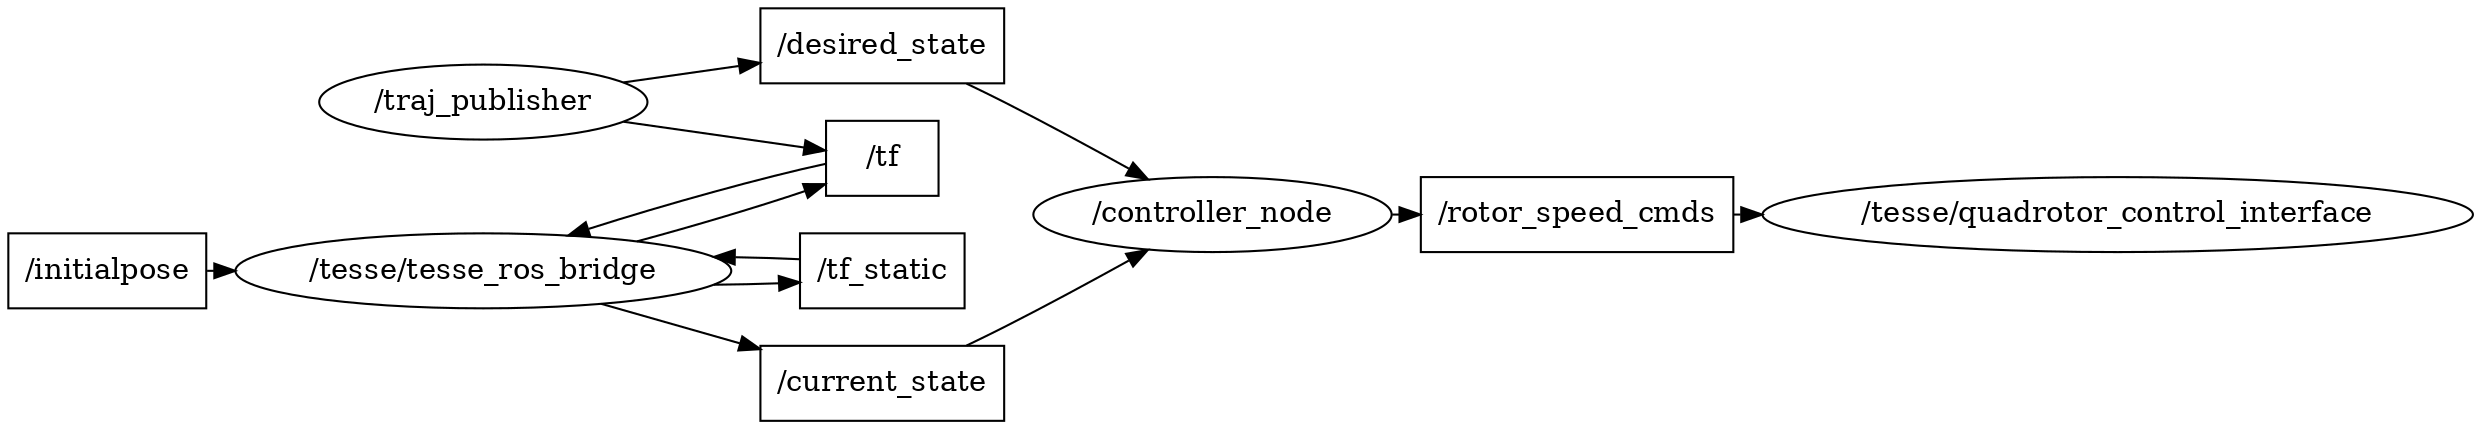
\includegraphics[width=\linewidth]{../results/screenshots/rqt_graph.png}
\caption{Node graph during circle tracking: the controller reads the desired and
current states and drives the simulator through \texttt{/rotor\_speed\_cmds}.\protect\label{fig:graph}}
\end{figure*}

\begin{evidence}
\repo{lab3/results/screenshots/rqt_graph.png};
\texttt{rosnode info} and \texttt{rostopic hz} in
\repo{lab3/results/logs/ros_communication.txt}; frame test in
\repo{lab3/results/logs/frame_check.txt}.
\end{evidence}

\gradeditem{sec:ctrl}{Controller Implementation}{20}
The control law follows Lee et al.\cite{lee2010} with the lab's conventions.
The $z$ axes point up (the paper's point down, which flips the signs of gravity
and of $b_{3d}$); the body $x$ axis lies halfway between two arms, so the
rotor map is the $F$ of \cref{sec:d2} with the simulator's rotor numbering
instead of the paper's eq.~(1); and $c_{\tau f}=c_d/c_f$. Each cycle computes
\begin{gather*}
e_x=x-x_d,\quad e_v=v-v_d,\quad A=-k_x e_x-k_v e_v+mg\,e_3+m\ddot x_d,\\
b_{3d}=\frac{A}{\lVert A\rVert},\quad
b_{2d}=\frac{b_{3d}\times b_{1c}}{\lVert b_{3d}\times b_{1c}\rVert},\quad
b_{1d}=b_{2d}\times b_{3d},\\
R_d=[\,b_{1d}\;b_{2d}\;b_{3d}\,],\quad
e_R=\tfrac12\left(R_d^\top R-R^\top R_d\right)^{\vee},\quad e_\Omega=\Omega,\\
f=A\cdot Re_3,\quad M=-k_R e_R-k_\Omega e_\Omega+\Omega\times J\Omega,\\
u=F^{-1}\begin{bmatrix}f\\M\end{bmatrix},\quad \omega_i=\operatorname{sign}(u_i)\sqrt{|u_i|},
\end{gather*}
with $b_{1c}=(\cos\psi_d,\sin\psi_d,0)$. As the template allows, the terms with the
desired angular velocity $\Omega_d$ and its derivative are dropped
($e_\Omega=\Omega$); \cref{sec:yaw} shows what this costs. The core of Part~5:

\begin{lstlisting}[style=code, basicstyle=\ttfamily\scriptsize]
const double l = d * cf / sqrt(2.0);   // rotors 1..4 in body quadrants I..IV
F2W << cf, cf, cf, cf,   l, l, -l, -l,   -l, l, l, -l,   cd, -cd, cd, -cd;

const Eigen::Vector3d thrust_des = -kx * ex - kv * ev + m * g * e3 + m * ad;
const Eigen::Vector3d b3d = thrust_des.normalized();
const Eigen::Vector3d b1d_yaw(cos(yawd), sin(yawd), 0.0);
const Eigen::Vector3d b2d = b3d.cross(b1d_yaw).normalized();
const Eigen::Vector3d b1d = b2d.cross(b3d);
Eigen::Matrix3d Rd;  Rd << b1d, b2d, b3d;
er = 0.5 * Vee(Rd.transpose() * R - R.transpose() * Rd);
eomega = use_omega_d ? Eigen::Vector3d(omega - R.transpose() * omegad_world)
                     : omega;            // use_omega_d = false in Lab 3
const double f = thrust_des.dot(R * e3);
const Eigen::Vector3d M = -kr * er - komega * eomega + omega.cross(J * omega);
Eigen::Vector4d wrench;  wrench << f, M;
const Eigen::Vector4d w2 = F2W.inverse() * wrench;  // omega_i * |omega_i|
for (int i = 0; i < 4; ++i) cmd.angular_velocities[i] = signed_sqrt(w2(i));
\end{lstlisting}

The controller was first tested hovering at $(0,0,\SI{2}{m})$ with yaw
\SI{45}{\degree}, then on the circle. With the final gains
(\cref{fig:circle}), over \SI{40}{s} (three laps) the position error is
\SI{4.3}{cm} RMS and at most \SI{4.8}{cm}.
Most of it is a constant altitude offset: the mean altitude is \SI{1.958}{m}
instead of \SI{2.000}{m}. The offset comes from the control law, which has no
integral term. In the 14 hover runs that settled (three others oscillated) the
sag times $k_x$ lies between \SI{0.36}{N} and \SI{0.42}{N} (for $k_x=1$ the sag is
\SI{36}{cm}, for $k_x=20$ \SI{1.8}{cm}): a constant force of about 4\,\% of the
weight is missing from the model, for instance through a slightly different mass or thrust coefficient,
and the position ``spring'' $k_x$ stretches until it supplies that force.

\begin{figure*}[h]
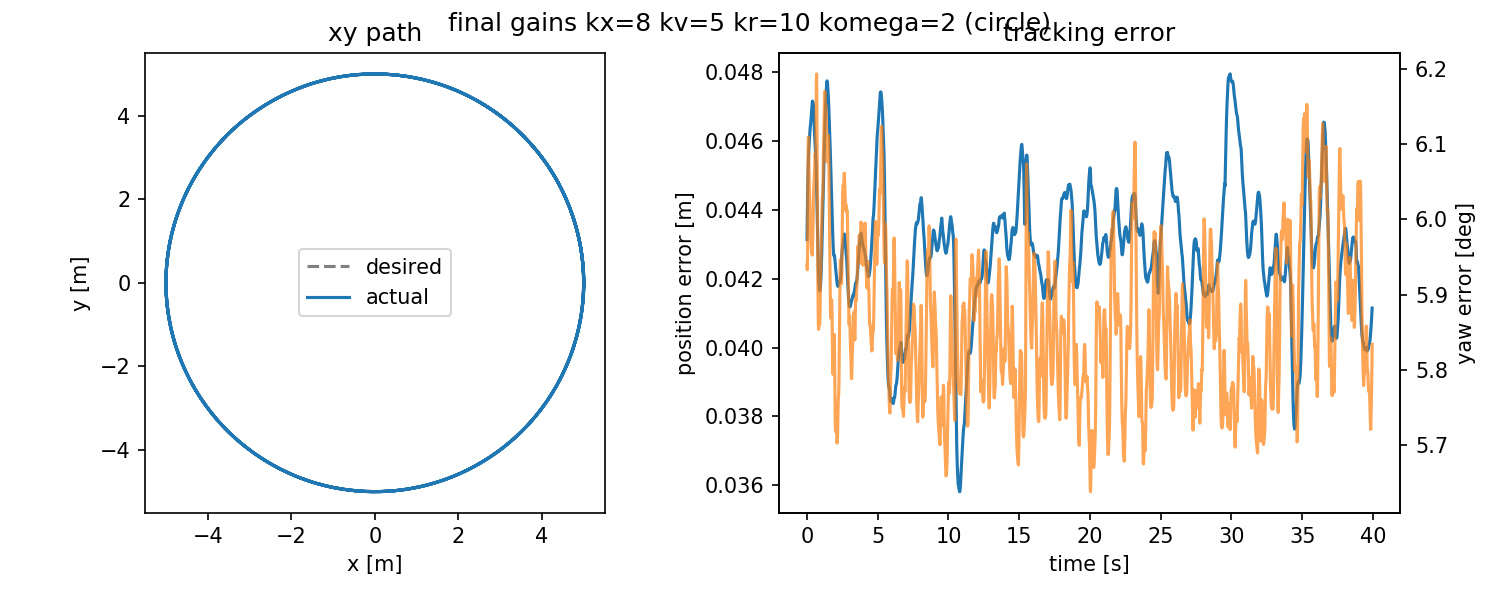
\includegraphics[width=0.8\linewidth]{../results/plots/final_circle.png}
\caption{Final gains on the circle. Left: desired and actual paths, which coincide
at this scale. Right: position error (blue, left axis) and yaw error (orange,
right axis) over \SI{40}{s}.\protect\label{fig:circle}}
\end{figure*}

\begin{evidence}
\repo{lab3/controller_pkg/src/controller_node.cpp}; run summary
\repo{lab3/results/logs/final_circle_summary.txt}; one lap in RViz,
\repo{lab3/results/video/rviz_circle.mp4}; simulator view
\repo{lab3/results/screenshots/sim_circle.png}.
\end{evidence}

\gradeditem{sec:yaw}{Rotation of \texttt{av-desired}}{10}
\texttt{traj\_publisher} broadcasts the desired pose as the TF frame
\texttt{av-desired}; its yaw turns at a constant \SI{-0.5}{rad/s} while the frame
moves round the circle. The grading item can be read in two ways, and both are
shown: the frame rotates as it moves (\cref{fig:rviz}), and the drone's own
frame \texttt{base\_link\_gt} rotates with it (\cref{fig:yaw}).
Over \SI{40}{s} the desired yaw turns by \SI{-1144}{\degree} and the drone
follows with a constant offset of \SI{5.86 \pm 0.10}{\degree}.

\begin{figure*}[h]
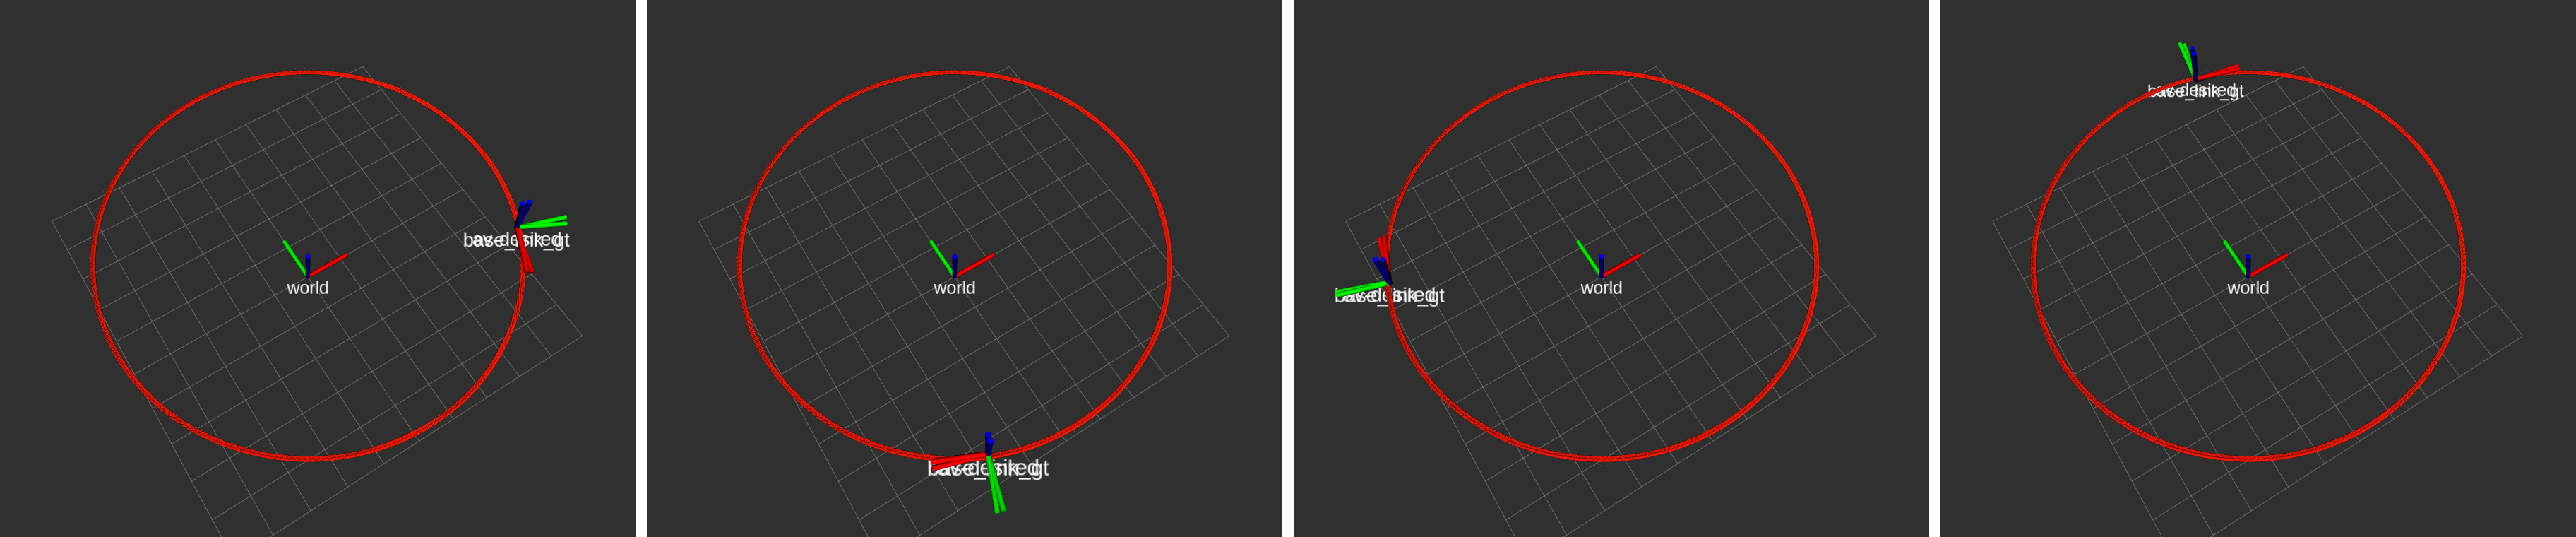
\includegraphics[width=\linewidth]{figures/rviz_quarters.png}
\caption{RViz top view at four points of one lap. \texttt{av-desired} and
\texttt{base\_link\_gt} overlap, so their labels print on top of each other; the
red $x$ axis of the pair turns with the position on the circle.\protect\label{fig:rviz}}
\end{figure*}

The offset follows from the control law. With $e_\Omega=\Omega$, a drone that
turns at the desired rate still meets the damping torque $-k_\Omega\Omega_z$,
which in steady state the attitude term must balance; for a pure yaw error
$\Delta\psi$ the yaw component of $-k_Re_R$ is $-k_R\sin\Delta\psi$. Hence
\begin{equation*}
\sin\Delta\psi=\frac{k_\Omega\,|\dot\psi_d|}{k_R}.
\end{equation*}
This predicts \SI{5.74}{\degree} for the final gains (measured \SI{5.86}{\degree})
and \SI{3.82}{\degree} for $(20,7,30,4)$ (measured \SI{3.99}{\degree}); the small
remainder is consistent with some yaw drag in the simulator. Feeding $\Omega_d$
forward, $e_\Omega=\Omega-R^\top R_d\Omega_d$, removes the lag; it was added as the
option \texttt{use\_omega\_d} for Lab~4.

\begin{figure}[h]
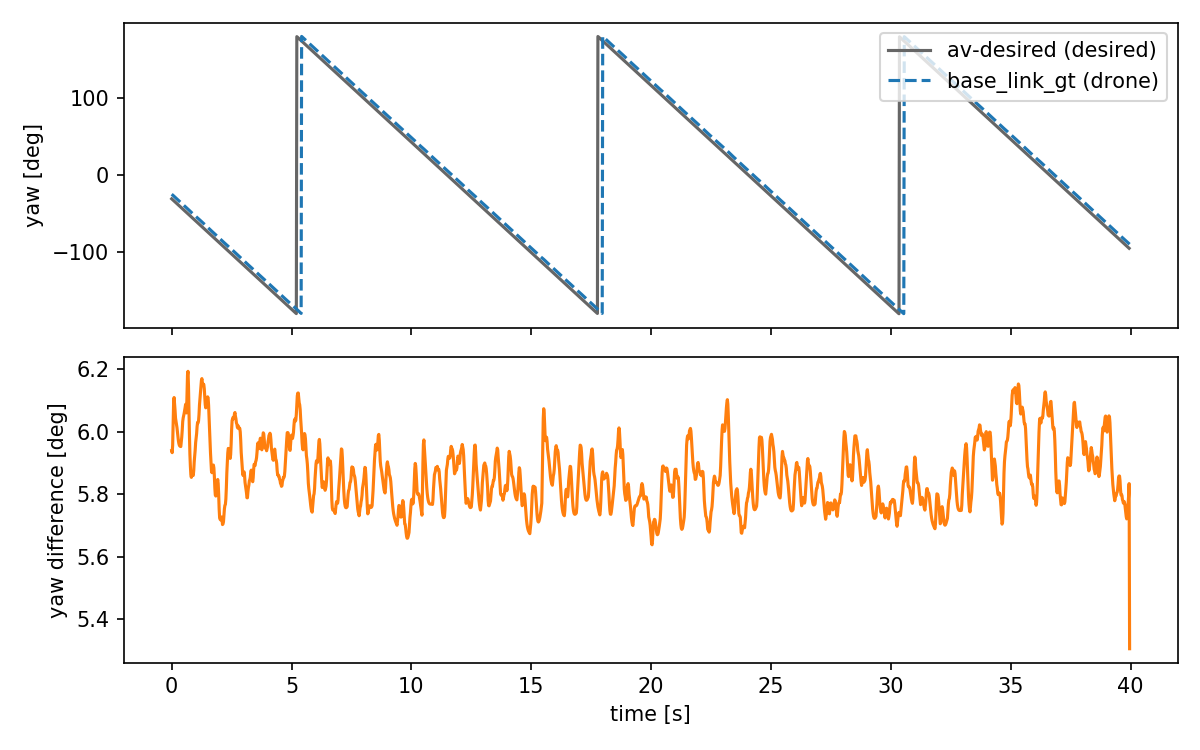
\includegraphics[width=0.75\linewidth]{../results/plots/av_desired_yaw.png}
\caption{Top: yaw of \texttt{av-desired} and of the drone (wrapped to
$\pm\SI{180}{\degree}$). Bottom: their difference.\protect\label{fig:yaw}}
\end{figure}

\begin{evidence}
\texttt{rviz\_q1..q4.png} in \repo{lab3/results/screenshots};
\repo{lab3/results/logs/av_desired_yaw.txt} and
\repo{lab3/results/logs/av_desired_yaw_oldgains.txt}.
\end{evidence}

\gradeditem{sec:tune}{Gain Tuning}{10}
A script respawned the drone, flew it with given gains, recorded a rosbag and
scored the run; 36 runs were logged, 17 hovering and 19 on the circle.
Besides the tracking error the score includes smoothness: the jitter (RMS of roll
and pitch minus their \SI{0.5}{s} moving average), the RMS step between
consecutive rotor commands, and the mean rotor speed. Hovering needs about
$\sqrt{mg/4c_f}\approx\SI{50}{rad/s}$ per rotor, so a much lower mean means that
the commands keep changing sign.
\begin{enumerate}
\item \emph{Hover, inner loop.} With $k_x=k_v=1$, raising $k_R$ from 1 to 20 left
the \SI{36}{cm} sag unchanged, since the two loops do different jobs;
$k_\Omega=5$ made the rotor commands swing between $\pm\SI{970}{rad/s}$, negative
half of the time.
\item \emph{Hover, outer loop.} Raising $k_x$ cut the sag as $1/k_x$
(\cref{sec:ctrl}). A stronger outer loop needs a faster inner one: with
$(k_x,k_v)=(10,5)$ the drone swung at \SI{1}{Hz} with $(k_R,k_\Omega)=(10,1)$ and
held its position to \SI{3.6}{cm} with $(20,3)$.
\item \emph{Circle, round one}, scored on the tracking error alone: the error kept
falling as all gains rose, and the best set, $(20,7,30,4)$, reached \SI{1.8}{cm}
RMS in a \SI{40}{s} run.
\item \emph{Round two}, scored on error and smoothness: $(20,7,30,4)$ jitters
\SI{1.39}{\degree} in pitch and its rotors average \SI{17.8}{rad/s}, so they keep
reversing, which a real motor cannot do. The final gains cut the jitter to
\SI{0.26}{\degree} and keep the rotors near the hover speed, at the cost of
\SI{2.5}{cm} more error (\cref{tab:tune}).
\end{enumerate}

\begin{table}[h]
\small
\begin{tabular}{@{}lrrrr@{}}
\toprule
$(k_x,k_v,k_R,k_\Omega)$ & error & jitter & step & mean \\
 & cm & deg & rad/s & rad/s \\
\midrule
$(1,1,1,1)$ template & diverges & -- & -- & -- \\
$(20,7,30,4)$ round one & 1.8 & 1.39 & 80.3 & 17.8 \\
$(8,5,10,2)$ final & 4.3 & 0.26 & 21.0 & 46.4 \\
\bottomrule
\end{tabular}
\caption{Circle runs of \SI{40}{s}: position error RMS, pitch jitter, rotor
command step RMS and mean rotor speed. With the template gains the drone leaves the
circle (error \SI{25}{m} RMS).\protect\label{tab:tune}}
\end{table}

\begin{evidence}
All runs in \repo{lab3/results/logs/tuning.txt}; smoothness in
\repo{lab3/results/logs/jitter_comparison.txt}; round-one and final gains side by
side in \repo{lab3/results/video/sim_old_vs_new.mp4}; a batch discarded for
lack of respawns, \repo{lab3/results/logs/tuning_invalid_no_respawn.txt}.
\end{evidence}

\section{Personal Reflection}\label{sec:reflection}
What I take from this lab is how a quadrotor moves at all. Its four rotors can
only push along the body $z$ axis: changing their speeds changes how hard they push
and at which corner, but never produces a force along $x$ or $y$. To move in the
horizontal plane the drone therefore has to tilt first, so that part of the thrust
points the way it should go while the vertical part still balances gravity, and
only then can it fly forward steadily. This is also why the controller works in two
stages, the position part choosing where the thrust should point and the attitude
part tilting the body to point it there. Nothing in the experiment contradicted
this picture.

For a real drone I would add a limit that the simulator does not impose: the rotor
speeds must not get too low. Each rotor has to keep spinning fast enough to carry
its share of the weight, about \SI{50}{rad/s} here, and running a motor at very low
speed, let alone reversing it, would hurt its performance and its lifetime. By this
measure the round-one gains $(20,7,30,4)$ would be unusable, since their rotors
averaged \SI{17.8}{rad/s} and kept reversing, while with the final gains the rotors
stay close to the hover speed.

\section{Discussion and Conclusions}\label{sec:conclusions}
\marginnote{Problems met under WSLg: windows show on the Windows desktop only when
WSL is started from the desktop session; the respawn key reaches Unity only
through \texttt{xdotool key -{}-window}; \texttt{ffmpeg -f x11grab} records black
frames, so videos were assembled from frames grabbed window by window; and the
bridge scripts needed \texttt{python3} first lines.}
With gains chosen on error and smoothness the controller tracks the circle with
\SI{4.3}{cm} RMS error and smooth rotor commands. The law has no integral term, which leaves
the \SI{4}{cm} altitude offset; an integral of $e_x$ in $A$ would remove it.

{\footnotesize\bibliography{refs}}
\bibliographystyle{plainnat}

\end{document}
